\documentclass[aspectratio=43]{beamer}
% Theme works only with a 4:3 aspect ratio
\usetheme{CSCS}

\usepackage{tikz}
\usepackage{pgfplots}
\usepackage{pgfplotstable}
\usetikzlibrary{pgfplots.groupplots,spy,patterns}
\usepackage{listings}
\usepackage{color}
\usepackage{tcolorbox}
\usepackage{anyfontsize}
\usepackage{xspace}
\usepackage{graphicx}

% define footer text
\newcommand{\footlinetext}{CUDA MiniApp}

% Select the image for the title page
\newcommand{\picturetitle}{cscs_images/image5.pdf}

% fonts for maths
\usefonttheme{professionalfonts}
\usefonttheme{serif}

% source code listing
\newcommand{\axpy}{{\ttfamily axpy}\xspace}

% set indent to a more reasonable level (so that itemize can be used in columns)
\setlength{\leftmargini}{20pt}

%\lstset{
%    language=[ANSI]C++,
%    basicstyle=\lstinlinefont{blue!30!black},
%    breaklines=true
%}
\lstdefinestyle{terminal}{
    showstringspaces=false,
    backgroundcolor=\color{white},
    basicstyle=\lstfont{black},
    identifierstyle=\lstfont{black},
    keywordstyle=\lstfont{black},
    numberstyle=\lstfont{black},
    stringstyle=\lstfont{black},
    commentstyle=\lstfont{black},
    emph={
        aprun, make
    },
    emphstyle={\lstfont{black}},
    breaklines=true
}

\lstset{
    language=[ANSI]C++,
    showstringspaces=false,
    backgroundcolor=\color{white!10!black},
    basicstyle=\lstfont{white},
    identifierstyle=\lstfont{white},
    keywordstyle=\lstfont{magenta!40!white},
    numberstyle=\lstfont{white},
    stringstyle=\lstfont{cyan},
    commentstyle=\lstfont{yellow!30!white},
    moredelim=[is][\lstfont{green!50!white}]{@}{@},
    emph={
        cudaMalloc, cudaFree,
        cudaMallocHost, cudaFreeHost,
        cudaMemcpyAsync, cudaMemcpy, cudaMemcpyHostToDevice, cudaMemcpyDeviceToHost,
        cudaSuccess, cudaGetLastError, cudaGetErrorString,
        cudaErrorMemoryAllocation, cudaError_t,
        cudaOccupancyMaxPotentialBlockSize,
        __global__, __shared__, __device__, __host__,
        __syncthreads,
        cudaEvent_t, cudaStream_t,
        cudaEventCreate, cudaEventSynchronize, cudaEventDestroy,
        cudaEventElapsedTime, cudaEventQuery, cudaEventRecord,
        cudaStreamWaitEvent,
        threadIdx, blockIdx, blockDim, gridDim,
        cudaStream_t, cudaStreamCreate, cudaStreamDestroy,
        cudaMemcpyDeviceToDevice, cudaMemcpyHostToHost,
    },
    emphstyle={\lstfont{green!50!white}},
    breaklines=true
}

\definecolor{codenumber}{rgb}{0.5,0.5,0.5}
\definecolor{codekeyword}{rgb}{0.9,0.4,0.7}
\definecolor{codeCUDA}{rgb}{1.0,0.6,0.6}

\lstdefinestyle{boxcuda}{
    language=[ANSI]C++,
    showstringspaces=false,
    backgroundcolor=\color{white!10!black},
    basicstyle=\lstfont{white},
    identifierstyle=\lstfont{white},
    keywordstyle=\lstfont{magenta!40!white},
    numberstyle=\lstfont{white},
    stringstyle=\lstfont{cyan},
    commentstyle=\lstfont{yellow!30!white},
    moredelim=[is][\lstfont{green!50!white}]{@}{@},
    emph={
        cudaMalloc, cudaFree,
        cudaMallocHost, cudaFreeHost,
        cudaMemcpyAsync, cudaMemcpy, cudaMemcpyHostToDevice, cudaMemcpyDeviceToHost,
        cudaSuccess, cudaGetLastError, cudaGetErrorString,
        cudaErrorMemoryAllocation, cudaError_t,
        cudaOccupancyMaxPotentialBlockSize,
        __global__, __shared__, __device__, __host__,
        __syncthreads,
        cudaEvent_t, cudaStream_t,
        cudaEventCreate, cudaEventSynchronize, cudaEventDestroy,
        cudaEventElapsedTime, cudaEventQuery, cudaEventRecord,
        cudaStreamWaitEvent,
        threadIdx, blockIdx, blockDim, gridDim,
        cudaStream_t, cudaStreamCreate, cudaStreamDestroy,
        cudaMemcpyDeviceToDevice, cudaMemcpyHostToHost,
    },
    emphstyle={\lstfont{green!50!white}},
    breaklines=true
}

\lstdefinestyle{boxcudatiny}{
    language=[ANSI]C++,
    showstringspaces=false,
    backgroundcolor=\color{white!10!black},
    basicstyle=\lsttinyfont{white},
    identifierstyle=\lsttinyfont{white},
    keywordstyle=\lsttinyfont{magenta!40!white},
    numberstyle=\lsttinyfont{white},
    stringstyle=\lsttinyfont{cyan},
    commentstyle=\lsttinyfont{yellow!30!white},
    moredelim=[is][\lsttinyfont{green!50!white}]{@}{@},
    emph={
        cudaMalloc, cudaFree,
        cudaMallocHost, cudaFreeHost,
        cudaMemcpyAsync, cudaMemcpy, cudaMemcpyHostToDevice, cudaMemcpyDeviceToHost,
        cudaSuccess, cudaGetLastError, cudaGetErrorString,
        cudaErrorMemoryAllocation, cudaError_t,
        cudaOccupancyMaxPotentialBlockSize,
        __global__, __shared__, __device__, __host__,
        __syncthreads,
        cudaEvent_t, cudaStream_t,
        cudaEventCreate, cudaEventSynchronize, cudaEventDestroy,
        cudaEventElapsedTime, cudaEventQuery, cudaEventRecord,
        cudaStreamWaitEvent,
        threadIdx, blockIdx, blockDim, gridDim,
        cudaStream_t, cudaStreamCreate, cudaStreamDestroy,
        cudaMemcpyDeviceToDevice, cudaMemcpyHostToHost,
    },
    emphstyle={\lstfont{green!50!white}},
    breaklines=true
}

\DeclareTextFontCommand{\emph}{\bfseries\color{blue!70!black}}

% Please use the predifined colors:
% cscsred, cscsgrey, cscsgreen, cscsblue, cscsbrown, cscspurple, cscsyellow, cscsblack, cscswhite

\author{Ben Cumming, CSCS}
\title{Introduction to the Summer School MiniApp}
\subtitle{}
\date{\today}

\begin{document}

% TITLE SLIDE
\cscstitle

%%%%%%%%%%%%%%%%%%%%%%%%%%%%%%%%%%%%%%%%%%%%
\begin{frame}[fragile]{Overview}
%%%%%%%%%%%%%%%%%%%%%%%%%%%%%%%%%%%%%%%%%%%%
    In this session we will cover:
    \begin{enumerate}
        \item What is a miniapp?
        \item The summer school miniapp overview.
        \item First look at the code.
        \item Compile, run and visualize the miniapp.
    \end{enumerate}
\end{frame}

%%%%%%%%%%%%%%%%%%%%%%%%%%%%%%%%%%%%%%%%%%%%
\begin{frame}[fragile]{What is a HPC miniapp?}
%%%%%%%%%%%%%%%%%%%%%%%%%%%%%%%%%%%%%%%%%%%%
    \begin{itemize}
        \item Full HPC applications are complicated.
        \begin{itemize}
            \item Difficult to model/understand performance behavior.
        \end{itemize}
        \item A miniapp is a smaller code that aim to characterize performance of larger applications.
        \begin{itemize}
            \item simpler to understand and benchmark than full applications.
            \item can be used to test different hardware, languages and libraries.
            \item good for learning new techniques!
        \end{itemize}
    \end{itemize}
\end{frame}

%%%%%%%%%%%%%%%%%%%%%%%%%%%%%%%%%%%%%%%%%%%%
\begin{frame}[fragile]{The Summer School Miniapp}
%%%%%%%%%%%%%%%%%%%%%%%%%%%%%%%%%%%%%%%%%%%%
    \begin{itemize}
        \item Throughout the summer school we will be using a  miniapp to reinforce the lessons.
        \begin{itemize}
            \item During talks there will be small programming exercises to  test out what you learn.
            \item Then you will get the opportunity to apply the techniques  to the miniapp.
        \end{itemize}
        \item We will start with a serial version that has no parallel  optimizations.
        \item By the end of the course we will have different  versions, one for each technique.
    \end{itemize}
\end{frame}

%%%%%%%%%%%%%%%%%%%%%%%%%%%%%%%%%%%%%%%%%%%%
\begin{frame}[fragile]{The Application}
%%%%%%%%%%%%%%%%%%%%%%%%%%%%%%%%%%%%%%%%%%%%
    \begin{itemize}
        \item The code solves \emph{Fisher's equation}, a \emph{reaction diffusion} model:
        \begin{equation*}
            \frac{\partial s}{\partial t} = D\left( \frac{\partial ^2s}{\partial x^2} + \frac{\partial ^2s}{\partial y^2} \right) + Rs(1-s).
        \end{equation*}
        \item Used to simulate travelling waves and simple  population dynamics.
        \begin{itemize}
            \item The species $s$ diffuses.
            \item The species reproduces to a maximum of $s=1$.
        \end{itemize}
    \end{itemize}
\end{frame}

%%%%%%%%%%%%%%%%%%%%%%%%%%%%%%%%%%%%%%%%%%%%
\begin{frame}[fragile]{Initial and Boundary Conditions}
%%%%%%%%%%%%%%%%%%%%%%%%%%%%%%%%%%%%%%%%%%%%
    \begin{center}
        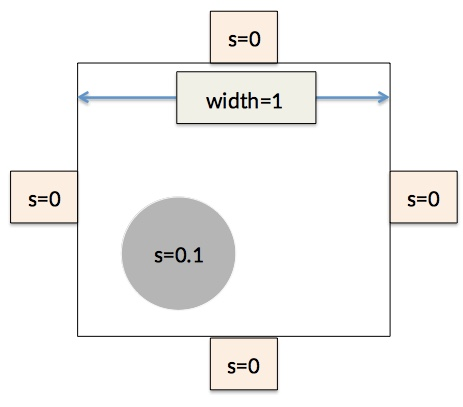
\includegraphics[width=0.5\textwidth]{./images/ic_bc.jpg}
    \end{center}
    The domain is rectangular, with fixed value of $s=0$ on  each boundary, and a circular region of $s=0.1$ in the
    lower left corner initially.
\end{frame}

%%%%%%%%%%%%%%%%%%%%%%%%%%%%%%%%%%%%%%%%%%%%
\begin{frame}[fragile]{Time Evolution of the Solution}
    \begin{center}
        $t=0.001$ \\
        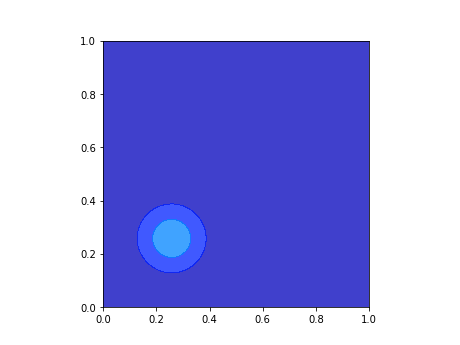
\includegraphics[width=0.6\textwidth]{./image_png/output001.png}
    \end{center}
\end{frame}

%%%%%%%%%%%%%%%%%%%%%%%%%%%%%%%%%%%%%%%%%%%%
\begin{frame}[fragile]{Time Evolution of the Solution}
    \begin{center}
        $t=0.005$ \\
        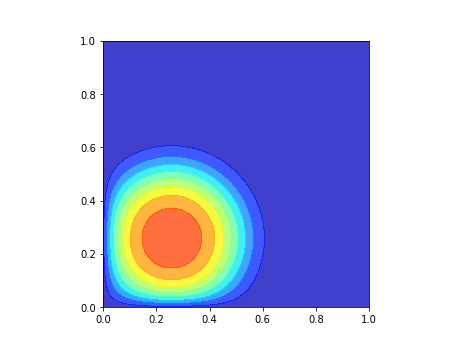
\includegraphics[width=0.6\textwidth]{./image_png/output005.png}
    \end{center}
\end{frame}

%%%%%%%%%%%%%%%%%%%%%%%%%%%%%%%%%%%%%%%%%%%%
\begin{frame}[fragile]{Time Evolution of the Solution}
    \begin{center}
        $t=0.01$ \\
        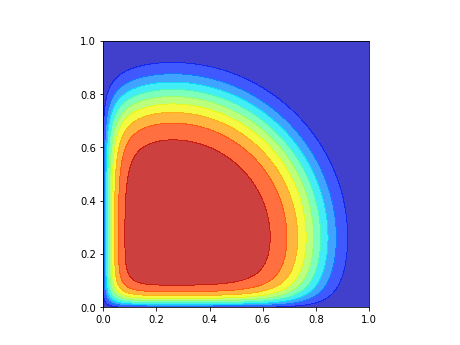
\includegraphics[width=0.6\textwidth]{./image_png/output01.png}
    \end{center}
\end{frame}

%%%%%%%%%%%%%%%%%%%%%%%%%%%%%%%%%%%%%%%%%%%%
\begin{frame}[fragile]{Time Evolution of the Solution}
    \begin{center}
        $t=0.02$ \\
        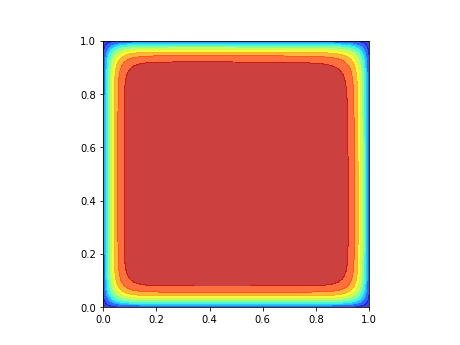
\includegraphics[width=0.6\textwidth]{./image_png/output02.png}
    \end{center}
\end{frame}

%%%%%%%%%%%%%%%%%%%%%%%%%%%%%%%%%%%%%%%%%%%%
\begin{frame}[fragile]{Numerical Solution}
%%%%%%%%%%%%%%%%%%%%%%%%%%%%%%%%%%%%%%%%%%%%
    \begin{itemize}
        \item The rectangular domain is discretized with a grid of  dimension $nx \times ny$ points.
        \item A finite volume discretization and method of lines gives the following ordinary differential equation for each grid point
        \begin{align}
            \frac{ds_{i,j}}{dt} =& \frac{D}{\Delta x^2} \left( -4s_{i,j} + s_{i+1,j}+ s_{i-1,j}+ s_{i,j+1}+ s_{i,j-1} \right) \nonumber\\
            &  + R s_{i,j}(1 - s_{i,j}) \nonumber
        \end{align}
        \begin{align}
            f_{ij} &= \left[ -(4+\alpha)s_{ij} + s_{i+1,j}+ s_{i-1,j}+ s_{i,j+1}+ s_{i,j-1} \right]^{k+1} + \alpha s_{ij}^{k}\nonumber \\
                   &=0 \nonumber
        \end{align}
            % TODO nonlinear equation to solve
    \end{itemize}
\end{frame}

%%%%%%%%%%%%%%%%%%%%%%%%%%%%%%%%%%%%%%%%%%%%
\begin{frame}[fragile]{Numeric Solution}
%%%%%%%%%%%%%%%%%%%%%%%%%%%%%%%%%%%%%%%%%%%%
    \begin{itemize}
        \item One nonlinear equation for each grid point:
        \begin{itemize}
            \item together they form a system of $N=nx \times ny$ equations
            \item solve with Newton's method
        \end{itemize}
        \item Each iteration of Newton's method solves a  linear system
        \begin{itemize}
            \item use a matrix-free Conjugate Gradient solver
        \end{itemize}
        \item Solve the nonlinear system at each time step
        \begin{itemize}
            \item requires in the order of between 5--10  conjugate  gradient iterations
        \end{itemize}
    \end{itemize}
\end{frame}

%%%%%%%%%%%%%%%%%%%%%%%%%%%%%%%%%%%%%%%%%%%%
\begin{frame}[fragile]{}
%%%%%%%%%%%%%%%%%%%%%%%%%%%%%%%%%%%%%%%%%%%%
    \begin{itemize}
        \item Don't worry if you don't understand everything.
            \item We don’t need a deep understanding of the  mathematics or domain problem to optimize the  code.
            \begin{itemize}
                \item I often work on codes with little domain knowledge.
            \end{itemize}
            \item The miniapp has a handful of kernels that can be  parallelized.
            \item And care was taken when designing it to make  parallelization as easy as possible.
            \item So let’s look a little closer at each part of the code\dots
    \end{itemize}
\end{frame}

%%%%%%%%%%%%%%%%%%%%%%%%%%%%%%%%%%%%%%%%%%%%
\begin{frame}[fragile]{The Code}
%%%%%%%%%%%%%%%%%%%%%%%%%%%%%%%%%%%%%%%%%%%%
    \begin{itemize}
        \item The application is written in \emph{C++}.
        \item It could be faster\dots
        \begin{itemize}
            \item We avoid aggressive optimization to make the code easier to understand.
            \item It is not a fine example of design.
        \end{itemize}
    \end{itemize}
\end{frame}

%%%%%%%%%%%%%%%%%%%%%%%%%%%%%%%%%%%%%%%%%%%%
\begin{frame}[fragile]{Code Walkthrough}
%%%%%%%%%%%%%%%%%%%%%%%%%%%%%%%%%%%%%%%%%%%%
    There are three main files of interest:
    \begin{enumerate}
        \item \lst{main.cpp}: Initialization and time stepping code.
        \item \lst{linalg.cpp}: BLAS level-1 vector-vector operations and conjugrate gradient solver.
        \item \lst{operators.cpp} The stencil kernel.
    \end{enumerate}
    The vector-vector kernels and diffusion operator  are the only kernels that have to be parallelized.
\end{frame}

%%%%%%%%%%%%%%%%%%%%%%%%%%%%%%%%%%%%%%%%%%%%
\begin{frame}[fragile]{Linear Algebra: linalg.cpp}
%%%%%%%%%%%%%%%%%%%%%%%%%%%%%%%%%%%%%%%%%%%%
    \begin{itemize}
        \item This file defines simple kernels for operatiing on vectors, e.g.:
        \begin{itemize}
            \item dot product $x^T y$ or $x\cdot y$: \lst{ss_dot}.
            \item linear combination $z=\alpha x + \beta y$: \lst{ss_lcomb}.
        \end{itemize}
        \item The kernels of interest are named \lst{ss_xxxx}.
        \item Each will have to be parallelized using CUDA, MPI and OpenACC.
        \item The \lst{ss_cg} function implements conjugate gradient using the vector and stencil operations.
    \end{itemize}
\end{frame}

%%%%%%%%%%%%%%%%%%%%%%%%%%%%%%%%%%%%%%%%%%%%
\begin{frame}[fragile]{Stencil operator: operators.cpp}
%%%%%%%%%%%%%%%%%%%%%%%%%%%%%%%%%%%%%%%%%%%%
    This file has the function that applies the stencil operator:

\begin{lstlisting}[style=boxcudatiny]
for i=2:nx-1
    for j=2:ny-1
        S(i,j) = -(4. + alpha) * U(i,j)
                                + U(i-1,j) + U(i+1,j)
                                + U(i,j-1) + U(i,j+1)
                                + alpha * x_old(i,j)
                                + dxs * U(i,j) * (1.0 - U(i,j));
    end
end
\end{lstlisting}
\end{frame}

%%%%%%%%%%%%%%%%%%%%%%%%%%%%%%%%%%%%%%%%%%%%
\begin{frame}[fragile]{Stencil operator: Interior grid points}
%%%%%%%%%%%%%%%%%%%%%%%%%%%%%%%%%%%%%%%%%%%%
    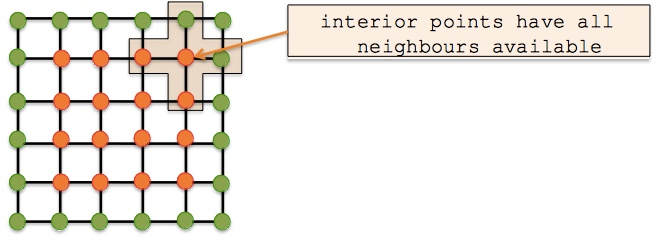
\includegraphics[width=\textwidth]{./images/grid_interior.jpg} \\
\begin{lstlisting}[style=boxcudatiny]
    S(i,j) = -(4+alpha)*U(i,j)
           + U(i-1,j) + U(i+1,j) + U(i,j-1) + U(i,j+1) + ...
\end{lstlisting}
\end{frame}

%%%%%%%%%%%%%%%%%%%%%%%%%%%%%%%%%%%%%%%%%%%%
\begin{frame}[fragile]{Stencil operator: Boundary grid points}
%%%%%%%%%%%%%%%%%%%%%%%%%%%%%%%%%%%%%%%%%%%%
    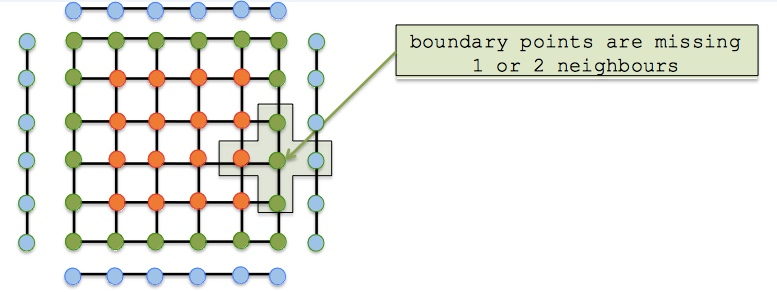
\includegraphics[width=\textwidth]{./images/grid_boundary.jpg} \\
    Points on the boundary need to use one or two external boundary points. \\
\begin{lstlisting}[style=boxcudatiny]
    S(i,j) = -(4+alpha)*U(i,j)
           + U(i-1,j) + bndE[j] + U(i,j-1) + U(i,j+1) + ...
\end{lstlisting}
\end{frame}

%%%%%%%%%%%%%%%%%%%%%%%%%%%%%%%%%%%%%%%%%%%%
\begin{frame}[fragile]{Testing the Code}
    Get the code and compile miniapp
\begin{lstlisting}[style=terminal]
> git clone git<at>github.com:eth-cscs/SummerSchool2019.git
> cd SummerSchool2019/miniapp/serial
> module load daint-gpu
> module swap PrgEnv-cray PrgEnv-gnu
> make
\end{lstlisting}
    Run the miniapp
\begin{lstlisting}[style=terminal]
> srun -Cgpu --reservation=course ./main 128 128 100 0.01
===================================================
Welcome to mini-stencil!
version   :: C++ serial
mesh      :: 128 * 128 dx = 0.00787402
time      :: 128 time steps from 0 .. 0.01
iteration :: CG 200, Newton 50, tolerance 1e-06
===================================================
---------------------------------------------------
simulation took 1.07502 seconds
7439 conjugate gradient iterations, at rate of 6919.88 iters/second
959 newton iterations
---------------------------------------------------
\end{lstlisting}
\end{frame}

%%%%%%%%%%%%%%%%%%%%%%%%%%%%%%%%%%%%%%%%%%%%
\begin{frame}[fragile]{Exercise: run the miniapp}
    \begin{itemize}
        \item Run with 4 different resolutions
        \begin{itemize}
            \item \lst{128 128 100 0.01}
            \item \lst{256 256 200 0.01}
            \item \lst{512 512 200 0.01}
            \item \lst{1024 1024 400 0.01}
        \end{itemize}
        \item For each case record:
        \begin{enumerate}
            \item the number of CG iterations.
            \item the number of CG iterations per second.
        \end{enumerate}
        \item We will refer to these results when testing the MPI and GPU versions of the code.
    \end{itemize}
\end{frame}

%%%%%%%%%%%%%%%%%%%%%%%%%%%%%%%%%%%%%%%%%%%%
\begin{frame}[fragile]{Exercise: visualize the reults}
    \begin{itemize}
        \item The application generates two data files with the final solution: \lst{output.bin} and \lst{output.bov}.
        \item There is a Python script that will show a contour plot  of the solution.
        \item Now is a good time to test if X-windows is working.
    \end{itemize}
\begin{lstlisting}[style=terminal]
> module load PyExtensions/2.7.15.1-CrayGNU-18.08
> python2 ../../scripts/plotting.py
\end{lstlisting}
\end{frame}

\cscschapter{Questions?}

\end{document}
